\chapter{GUI development}

Haskell has at least four toolkits for programming a graphical interface: wxHaskell, Gtk2Hs, hoc, and qtHaskell. However, Java Graphics APIs--AWT and Swing--provide a huge set of reusable GUI components, such as button, text field, label, panel and frame for building GUI applications. So, it is more flexible to develop a GUI by reusing these classes in Java. I believe it would also be an interesting work to implement a comprehensive GUI in Haskell. In this project, a useable and functional GUI is developed in Java. The GUI design is based on Sestoft's `lambda term reducer' which could be found at ``http://www.itu.dk/people/sestoft/lamreduce/'', and the draft report describing the implementation in Sestoft\cite{sestoft1996}. Some improvements have been made such as to deal with non-terminating terms in trace enviroment. In addition, the Curry type assignment system is also enable in the GUI which is run in parallel with $\lambda$-term reduction.    

\section{Layout}

\begin{figure}[ht]
\centering
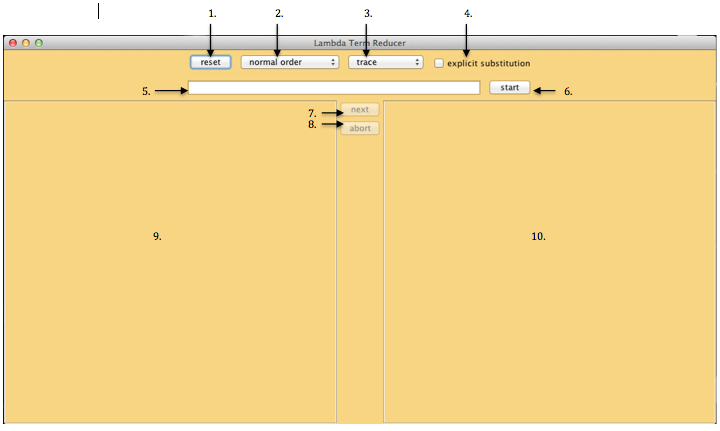
\includegraphics[width=\textwidth]{pics/GUILax}
\caption{Layout of the Graphical User Interface}
\label{fig:gui}
\end{figure}

\noindent The function of each button or text area label in Figure \ref{fig:gui}:
\begin{enumerate}
\item reset button: reset all the button, drop-down lists values to default and empty the output areas 9 and 10.
\item reduction strategy drop-down list: 5 reduction strategies can be selected by the user.
\item reduction step drop-down list: the user can select how the reduction is performed: normalize: directly output the reduction result by a specific reduction strategy and states how many $\beta$-reductions performed. trace: output the reduction procedure for each $\beta$-reduction performed. single step: it only outputs the reduction of a single step, moreover, the buttons 7 and 8 are enabled to let user choose whether continue reduction or abort the procedure.  
\item explicit substitution check box: user can tick to enable explicit substitution and garbage collection.
\item input field: user input the term to be reduced and typed in this field.
\item start button: press the button to start the procedure with pre-specifed reduction strategy(2) and reduction step option(3).
\item next button: carry on reduction when single step is selected.
\item abort button: abort the reduction when the input term is non-terminate or in the middle of single step reduction.
\item reduction output area: the output of reduction procedure is printed out in this area. The format is decided by the reduction step option(2).
\item type assignment output area: the output of type assignment result is printed out in this area. For normalize and trace, only the input term is typed. However, if the single step strategy is selected, intermediate terms during reduction would also be typed.
\end{enumerate}


\section{Functionalities}

In this section, the functionalities of the GUI would be shown by some sample runs. We mainly test the difference in different output environment: normalize, trace, and single-step. Moreover, the improvements compared to Sestoft's lambda term reducer would be shown by example. Here, we will not give any examples on the differences between outputs by different reduction strategies, since it has already been shown in Chapter 1. 

\subsection{Normalize}

\begin{figure}[ht]
\centering
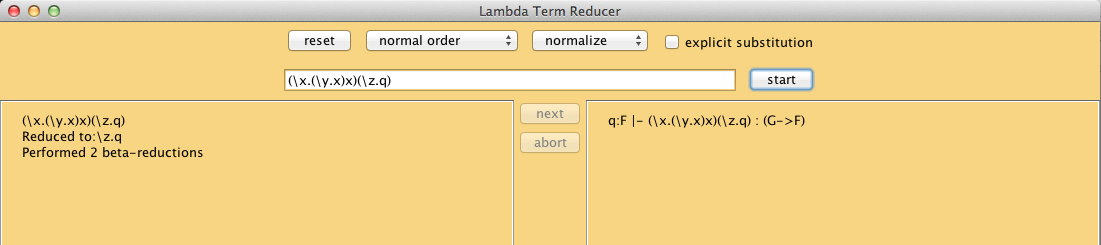
\includegraphics[width=\textwidth]{pics/normalize}
\caption{Sample run in normalize environment}
\label{fig:normalize}
\end{figure}

When `normalize' option is selected, the reducer tries to normalize the input $\lambda$-term with a specific reduction strategy. In other words, it reduces the input term with a reduction strategy until no more $\beta$-reduction can be performed. The intermediate terms and the reduction procedure would not be shown in this case. It outputs the final term reached and displays the total $\beta$-reduction performed. On the right output area, the type assignment result is displayed. It is displayed in the derivation format: context $\vdash$ statement, which means the statement is derivable from the context. Recall that, the context is used to collect all statements used for the free variables of a term when typing that term. In this example, only $q$ is free others are all bound. 

\subsection{Single-step}

The `single-step' option performs $\beta$-reduction once per time and user can control whether continue or abort. 

\begin{figure}[ht]
\centering
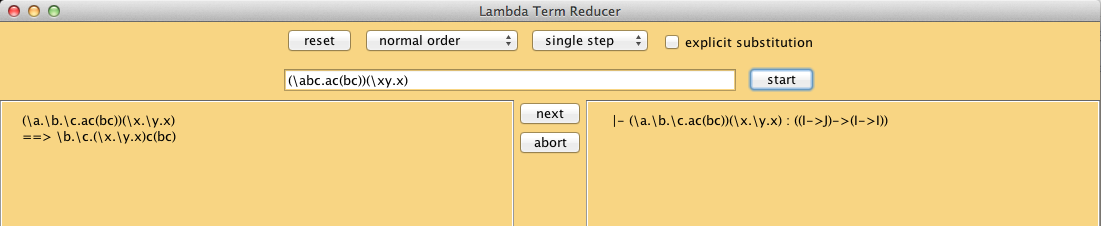
\includegraphics[width=\textwidth]{pics/single1}
\caption{Sample run in single-step environment}
\label{fig:s1}
\end{figure}

As shown in Figure \ref{fig:s1}, after the `start' button is pressed, a single $\beta$-reduction is performed and the corresponding type assignment result is displayed. As we can see, the `next' button and `abort' button are enabled now. The user can press the `next' button to perform another single $\beta$-reduction step, or press the `abort' button to abort the whole procedure.  

\begin{figure}[ht]
\centering
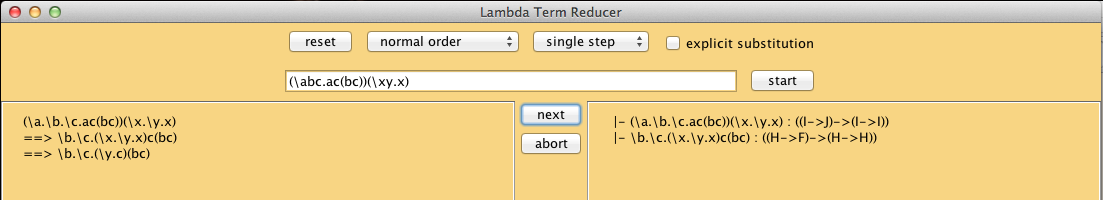
\includegraphics[width=\textwidth]{pics/single2}
\caption{Sample run in single-step environment--second step}
\label{fig:s2}
\end{figure}

Each time the `next' button is pressed, a single $\beta$-reduction would be performed until no reduction can be performed according to the reduction strategy. In Figure \ref{fig:s2}, another $\beta$-reduction is performed and the corresponding type assignment result is displayed. 

\begin{figure}[ht]
\centering
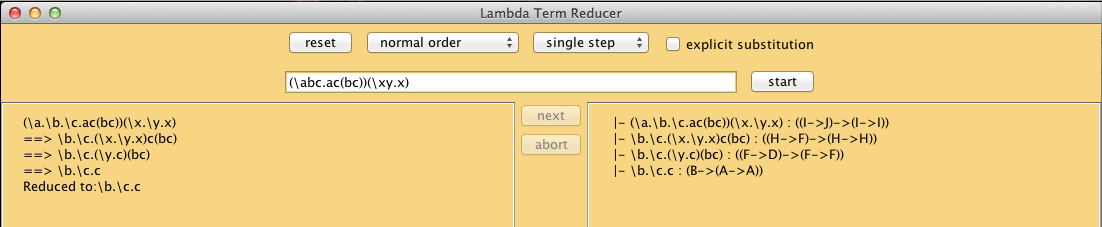
\includegraphics[width=\textwidth]{pics/single3}
\caption{Sample run in single-step environment--final result}
\label{fig:s3}
\end{figure}

When there is no $\beta$-reduction to perform on the $\lambda$-term, the reduction procedure stops and both `next' and `abort' buttons are disabled.

\subsection{Deal with non-terminating terms in trace environment}

In Sestoft's implementation, the engine enters an infinite loop and stuck when the input term is non-terminating and the output environment is `trace'. There is no intermediate terms or steps displayed, so the user would not know what is happending and what the problem is. In this project, when the input term is non-terminating and the tracer is `trace', all the intermediate steps would be displayed.   


\begin{figure}[ht]
\centering
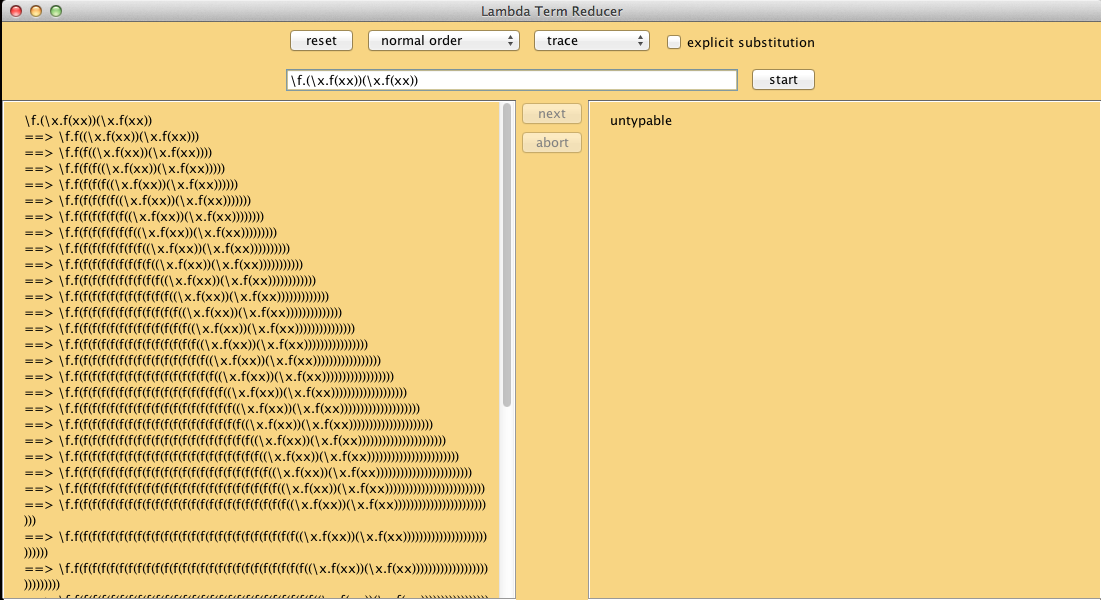
\includegraphics[width=\textwidth]{pics/nonterminate}
\caption{Sample run of a non-terminate term in trace environment}
\label{fig:nt}
\end{figure}

\subsection{Explicit Substitution}

\begin{figure}[ht]
\centering
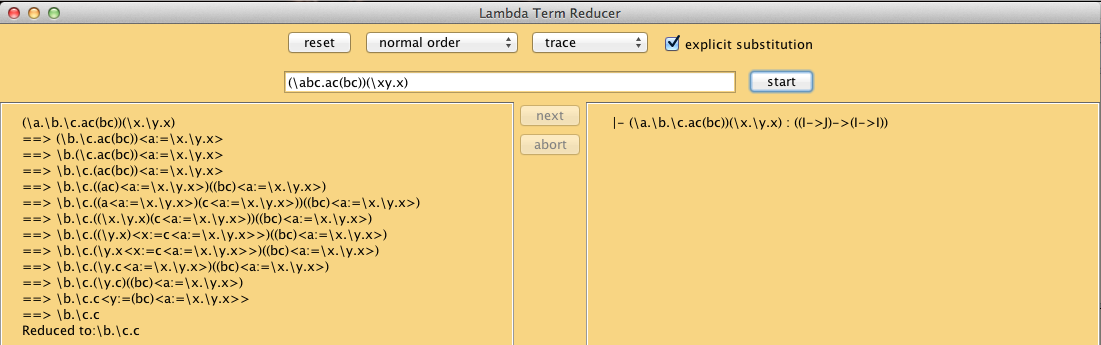
\includegraphics[width=\textwidth]{pics/explicit}
\caption{Sample run when explicit substitution enabled}
\label{fig:explicit}
\end{figure}

